\documentclass[12pt]{article}

\usepackage[a4paper, margin=1in]{geometry}
\usepackage{graphicx}
\usepackage[
    defernumbers=true,
    citestyle=authortitle,
    autocite=footnote
]{biblatex}
    \addbibresource{bibliography.bib}
\usepackage[
    colorlinks,
    linkcolor=black,
    citecolor=black,
    urlcolor=blue
]{hyperref}
\usepackage{float}
\usepackage{mdframed}
\usepackage{listings}
\usepackage{minted}
    \setminted{
        bgcolor=LightGray,
        linenos,
        frame=lines,
        framesep=5mm,
        fontsize=\footnotesize
    }
\usepackage[svgnames]{xcolor}

\newcommand{\code}[1]{\texttt{\color{Grey}#1}}

\setlength{\parskip}{1em}
\setlength{\parindent}{0em}

\title{Criterion C - Development}
\author{}
\date{}
\begin{document}

\maketitle

\section{Techniques Used}

\begin{enumerate}
    \item Classes
    \item Methods
    \item Encapsulation
    \item Graphical User Interface
    \item Constraint Programming
    \item Generators
    \item Lists
    \item Dictionaries
\end{enumerate}

\section{Structure}

\subsection*{Flowchart}

\begin{figure}[H]
    \centering
    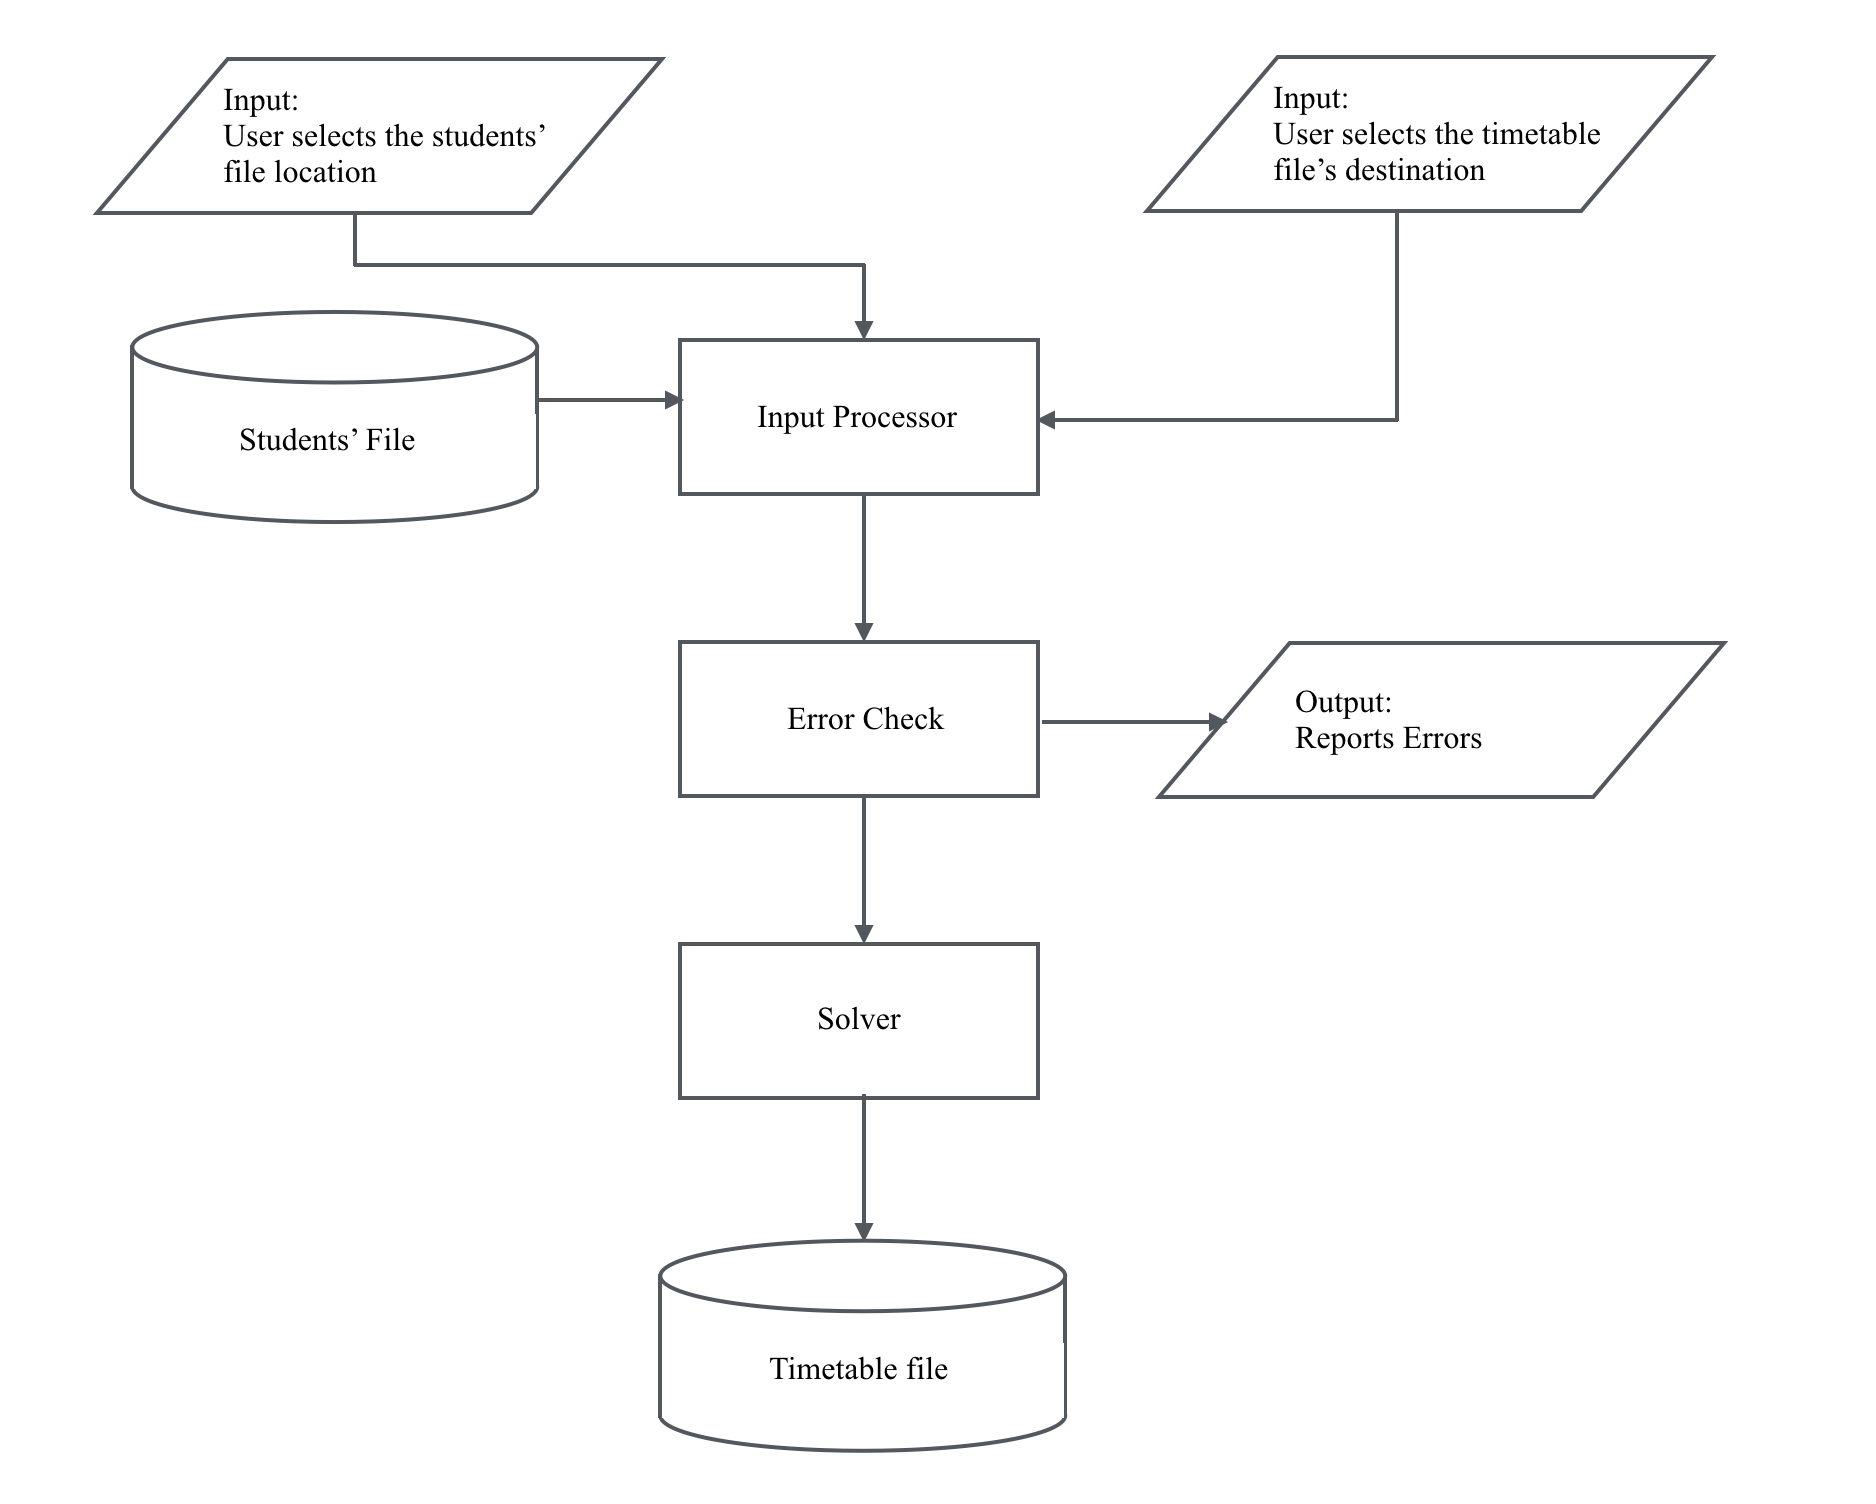
\includegraphics[width=\textwidth]{system_flowchart}
\end{figure}

\subsection*{Program Structure}

\begin{figure}[H]
    \label{fig:dir_structure}
    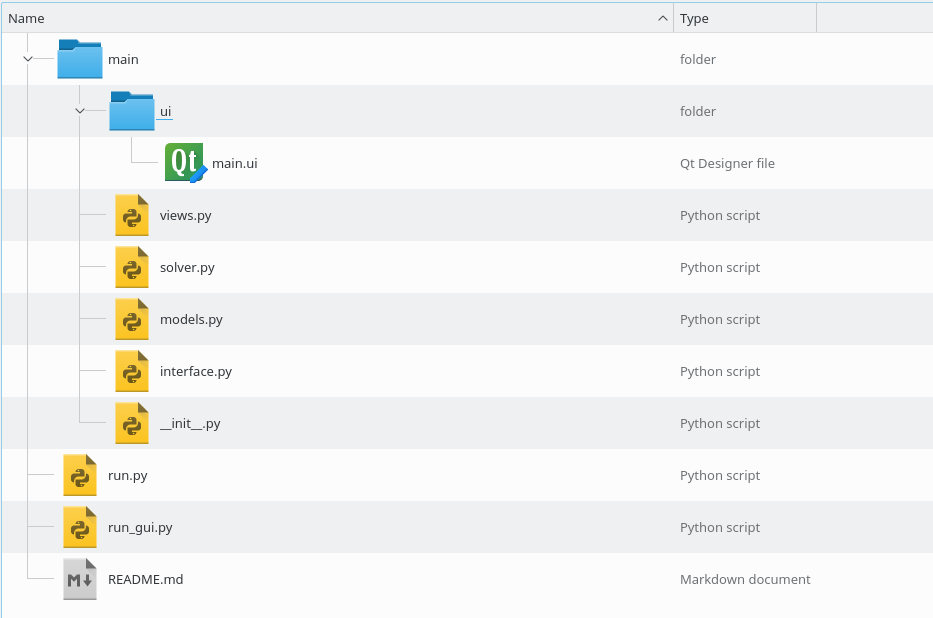
\includegraphics[width=\textwidth]{directory_structure}
\end{figure}

In \autoref{fig:dir_structure}, .py files contain python source code, main.ui contains qt
xml markup, which is contain the structure of the GUI windows, and README.md is a contains
basic information about the program and my contact information.

\section{Tools \& Software}

The application was made in Python 3, making use of a number of different software
libraries.  

The application was written using the Neovim \autocite{neovim} editor. The core solver of
the application --- responsible for creating the timetables, given the students and subjects
--- was made using Google's ortools \autocite{ortools} library, which was chosen for its
speed and reputable developer.  For reading the Excel spreadsheets, the
openpyxl\autocite{openpyxl} library was used, since it is the most used --- and therefore
best supported --- library for this purpose. The GUI of the program was made using the PyQt
framework as well as Qt Designer, for graphically designing the user interface. The
framework was chosen for its stability as well as for being compatible with multiple
operating systems. This was particularly important since I was developing the program on
Arch Linux while the client would eventually run it on Windows 7.


\section{How it works}

\subsection{Generators}

Generators are a feature of the python language that is used extensively in my program and
so, knowledge of them is necessary to understand the function of the program. 

"Generators functions allow you to declare a function that behaves like an iterator, i.e. it
can be used in a for loop."\autocite{generators}. When a function has to return a list of
values, it is usually much simpler to create a generator function than to directly return a
list. Consider the following example:
%
\begin{minted}{python}
def count(limit):
    i = 0
    while i <= limit:
        yield i
        i += 1

for num in count(5):
    print(num)
\end{minted}
%
This will output:\vspace{-5mm}
%
\begin{verbatim}
1
2
3
4
5
\end{verbatim}
%
When a function has the \code{yield} keyword inside it, it automatically becomes a
generator and can be used in a \code{for} loop like in the example. What happens in the
\code{for} loop in the example is the following: When the loop begins, the function is run
until a \code{yield} statement is found. Then, the loop variable (\code{i}) is set to
the value passed to \code{yield} statement (which is 0 for the first iteration), and the
body of the loop is executed. Control is passed back to the generator, and line 5 is
executed, the generator keeps control until another yield statement is hit (which will be on
line 4, since we are in a \code{while} loop in the generator), and the cycle continues.
When either a \code{return} statement or (in this case) the end of the generator is hit,
the loop stops.

\subsection{Loading and parsing the students' file}

The data the program needs is stored in an Excel file with the following structure:

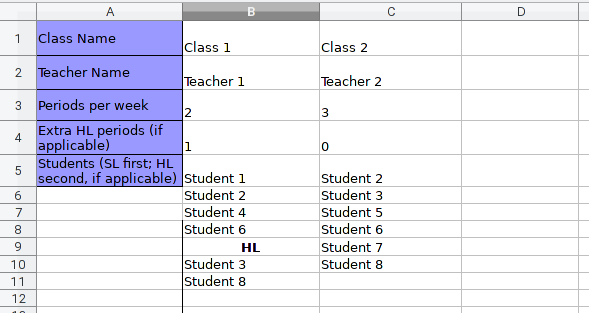
\includegraphics[width=\textwidth]{data_file_structure.png}

In the program, the Datastore class (diagram below) is responsible for loading
the file and providing the data in a usable format.
%
\begin{table}[H]
    \centering
    \def\arraystretch{1.5}
    \begin{tabular}{|l r|}
        \hline
        \multicolumn{2}{|c|}{Datastore}\\
        \hline
        \hline
        openpyxl.worksheet.Worksheet &worksheet\\
        \hline
        Generator[Subject] &getSubjects()\\
        Dict[str, List[Subject]] &getStudents(includeTeachers)\\
        \hline
    \end{tabular}
    \label{table:datastore}
\end{table}
%
The \code{worksheet} field stores the data of the excel worksheet as an openpyxl Worksheet
object. 

The \code{getSubjects} method is a generator returning all the subjects contained in the
worksheet as \code{Subject} objects:
\vspace{-3mm}
\inputminted{python}{datastore_get_subjects.py}

The \code{getStudents} method provides the subjects that each student has selected. This
information is provided as a dictionary with strings containing the students' names as keys,
each mapped to a list of \code{Subject} objects, representing the subjects the student is a
part of. The method also accepts the optional parameter \code{include\_teachers}. If
\code{True} is passed to this, then the teachers are also included in the output as if they
were students, with their subjects being the ones that they teach.
\vspace{-3mm}
\inputminted{python}{datastore_get_students.py}

\subsection{Solver}

The timetables are created using a technique called \emph{constraint programming}.
Generally, this is a method of finding possible values for a number of variables given a set
of values that each can take as well as a set of constraints for these variables, e.g. that
two can't take the same value or that they all have to add up to a specific number.  This is
achieved by assigning values to the variables until either a valid solution is reached or no
other values can be set without breaking a constraint, in which case the variables which
created the problem are unset and the algorithm continues from an earlier state were there
were no problems.

In order to use this technique it is necessary to model the problem being addressed using
the variables and constraints described. For my program I decided on the following model:
%
\begin{itemize}
    \item Each period to be present on the timetable is represented as one variable, taking
        an integer value between 0 and 19 (0 == Monday, first period, 19 == Friday, last
        period). So, taking Computer Science HL as an example, which is taught for 3 periods
        each week, there will be three variables: \textit{ComputerScienceHL-p1},
        \textit{ComputerScienceHL-p2} and \textit{ComputerScienceHL-p3}, each taking a value
        between 0 and 19.

    \item Each student (or teacher) is modelled as a constraint which does not allow the
        periods the person has to be present on to be on the same spot on the timetable,
        i.e. take the same numerical value. So, if, for example, Alice were to have taken
        Business SL and Computer Science HL, there would be a constraint, that would not
        allow the variables \textit{ComputerScienceHL-p1}, \textit{ComputerScienceHL-p2},
        \textit{ComputerScienceHL-p3} and \textit{BusinessSL-p1}, \textit{BusinessSL-p2} to
        take the same value.
\end{itemize}
%

Here is the function that handles creating the model and passing it to the solver, with
comments explaining it step-by-step.
\newpage
\inputminted{python}{solver_listing.py}

\printbibliography[type={software},title={Libraries}]
\printbibliography[type={online}, title={References}]
\end{document}


